\chapter{Policy Implementation and Evaluation in an IFC-enabled Browser}
\label{ch:eval}
\blfootnote{The content of this
  chapter is based partly on the work published as part of the paper,
  ``WebPol: Fine-grained Information Flow Policies for Web Browsers''~\cite{webpol}} 

This chapter describes the implementation of \sys~(Chapter~\ref{ch:webpol}) 
and the LIR policy (Chapter~\ref{ch:lir}) on top of
an existing IFC-instrumentation~\cite{just11PLASTIC,post14,csf15}. 
Their work instrumented WebKit, the browser engine used in Safari, for enforcing 
dynamic IFC in the three main components of the engine --- JavaScript 
bytecode interpreter, the document object model (DOM) engine, and the
event handling mechanism. 

Labels in their instrumentation are word size bit-sets (currently 64 
bits); each bit in the bit-set represents label from a distinct domain
(like google.com). Join on labels is simply bitwise or. Their
instrumentation adds labels to all data structures, including
registers, objects, object properties and scope chain pointers. They 
attach security labels to every node in the DOM graph and all its 
properties, including pointer to other nodes. 
They instrument the code to propagate explicit and implicit labels 
and implement the permissive-upgrade check. 

They instrument WebKit’s JavaScript bytecode interpreter (JavaScriptCore) 
for enforcing dynamic IFC for JavaScript~\cite{just11PLASTIC,post14}. 
In WebKit, bytecode is generated
by a source-code compiler and organized into code blocks. Each code
block is a sequence of bytecodes with line numbers and corresponds to
the instructions for a function or an \texttt{eval} statement. A code
block is generated when a function is created or an \texttt{eval} is
executed. Their instrumentation performs control flow analysis on a
code block when it is created and generates a CFG for it before it
starts executing. The IPDs of its nodes are calculated by static
analysis of its bytecode; they are computed using an algorithm by
Lengauer and Tarjan with CFG as an input to the
algorithm~\cite{Lengauer}. The formalization of the bytecodes, the
semantics of its bytecode interpreter with the instrumentation of
dynamic IFC, and the proof of correctness of instrumentation of the
bytecodes with the IFC semantics is shown in~\cite{post14Extended}.
Additionally, all native JavaScript methods in the Array, RegExp, 
and String objects are instrumented and appropriate  
IFC checks in the native C code implementing all DOM APIs up
to Level 3 are added~\cite{csf15}. 
They also modify the event handling loop, labeling every event and
event handler based on their formalization of the event handling loop
with the IFC checks~\cite{csf15}.  

Their work enforces IFC soundly in all the major components of 
a web browser while tracking labels at a fine-granularity. This thesis 
builds on top of their instrumentation for enforcing the ideas presented 
earlier. For exceptions, a synthetic exit node is added to the CFG
along with the edges as described earlier in
Section~\ref{sec:excsen}. Additional changes are required to the
compiler to make it compliant with the instrumentation. The
modification is to emit a slightly different, but functionally
equivalent bytecode sequence for \texttt{finally} blocks; 
this is needed for accurate computation of IPDs. 


\section{Implementation and Evaluation of \sys}
\label{sec:implpol}
\subsection{Implementation of \sys}
{\sys} is prototyped in WebKit on top of the prior IFC enforcement in
WebKit described above~\cite{just11PLASTIC,post14,csf15}. To implement
{\sys}, the HTML parser was modified to distinguish policy files
(extension \texttt{.policy}) from other JavaScript files and to give
policy code extra privileges. Two new JavaScript API functions ---
\texttt{setLabel()} and \texttt{setContext()} --- were added. Finally,
the event dispatch logic was modified to trigger policy handlers
before other handlers. In all, 25 lines in the code of the parser were
modified, 60 lines for the two new API functions were added and 110
lines in the event dispatch logic were modified. Thus, implementing
{\sys} has low overhead, and can be ported to other browsers easily.

\subsection{Evaluation of \sys}
\label{sec:eval-webpol}
The goal of the evaluation is two-fold. The first goal is to measure
the overhead of the system with IFC enforcement and {\sys}, both in
parsing and installing policies during page load and for executing
policy handlers later. This is done by running a few benchmarks, by measuring the
overhead for the examples presented in Chapter~\ref{sec:examples}, and
for two real-world websites. Second, to 
understand whether {\sys} can be used easily, {\sys} policies are
applied to two real-world websites. All the experiments were
performed on a 3.2GHz Quad-core Intel Xeon processor with 8GB RAM,
running Mac OS X version 10.7.4 using Safari 6.0. The implementation
and evaluation is done on WebKit nightly build $\#r122160$. As the
existing IFC instrumentation does not handle JIT, JIT support was
disabled in all the experiments. 

\subsubsection{Performance Overheads on Synthetic Examples}
To measure the instrumentation's runtime overhead, four examples from 
Chapter~\ref{sec:examples} (Examples~1,~2 and the two sub-examples of
Example~3) were tested in three different configurations:
\textbf{Base}---uninst\-ru\-mented browser, no enforcement;
\textbf{IFC}---existing instrumented browser with IFC checks, but no
policy handlers (everything is labeled public);
\textbf{{\sys}}---instrumented browser running policy handlers.

\newcolumntype{C}[1]{>{\centering\let\newline\\\arraybackslash\hspace{0pt}}m{#1}}

\begin{table}[tbp]
\centering
\begin{tabular}{ | C{2cm} || C{1.5cm} | C{1.5cm} | C{1.5cm} || C{1.5cm} | C{1.5cm} | C{1.5cm} |}
\hline
\multicolumn{1}{|c||}{ } &
\multicolumn{3}{ c ||}{JavaScript Execution Time} &
\multicolumn{3}{ c |}{Page Load Time} \\
\hline
 Example \# & \textbf{Base} & \textbf{IFC} & \textbf{\sys} & \textbf{Base} & \textbf{IFC} & \textbf{\sys} \\
  \hhline{|=#=|=|=#=|=|=|} 
  Example~1 & 2430 & 2918 (+20.1\%) & 2989 (+1.9\%) & 16 & 17 (+6.3\%) & 19 (+12.5\%) \\  
\hline
  Example~2 & 3443 & 4361 (+26.7\%) & 5368 (+29.2\%) & 41 & 43 (+4.9\%) & 46 (+7.2\%)\\ 
\hline
  Example~3 (count) & 1504 & 1737 (+15.5\%) & 1911 (+11.6\%) & 24 & 25 (+4.2\%) & 31 (+25.0\%) \\
\hline
  Example~3 (presence) & 1780 & 2095 (+17.7\%) & 2414 (+18.9\%) & 26 & 28 (+7.7\%) & 30 (+7.7\%)\\
\hline
\end{tabular}
\caption{Performance of examples from Section~\ref{sec:examples}. All
  time in ms. The numbers in parenthesis are additional overheads
  relative to \textbf{Base}.}
\label{table:eap}
\end{table}

\noindent
\textbf{JavaScript execution time:} The overheads of executing policy
handler code were measured by interacting with all four programs
manually by entering relevant data and performing clicks a fixed
number of times. For each of these configurations, the total time
spent \emph{only in executing JavaScript} was measured, including 
scripts and policies loaded initially with the page and the scripts
and policies executed in response to events. The difference between
\textbf{IFC} and \textbf{Base} run times is the overhead of dynamic
IFC, while the difference between the \textbf{\sys} and
\textbf{IFC} run times is the overhead of evaluating policy
handlers. Since only JavaScript execution time is measured and
there are no time-triggered handlers in these examples, variability in
the inter-event gap introduced by the human actor does not affect the
measurements.

The left half of Table~\ref{table:eap} shows these observations.
%
All numbers are averages of 5 runs and the standard deviations are
all below 7\%. %\TODO{Fill these numbers}
%
Taint-tracking (\textbf{IFC}) adds overheads ranging from 15.5\% to
26.7\% over \textbf{Base}. To this, policy handlers (\textbf{\sys})
adds overheads ranging from 1.9\% to 29.2\%. The \textbf{\sys}
overheads are already modest, but this is also a very challenging
(conservative) experiment for {\sys}. The scripts in 
both sub-examples of Example~3 do almost nothing. The scripts in
Examples~1 and Example~2 are slightly longer, but are still much
simpler than real scripts. On real and longer scripts, the relative
overheads of evaluating the policy handlers is significantly lower as
shown later. Moreover, the baseline in this experiment does not
include other browser costs, such as the cost of page parsing and
rendering, and network delays. Compared to those, both \textbf{IFC}
and \textbf{\sys} overheads are negligible.

\noindent
\textbf{Page load time:} The time taken for loading the initial page
(up to the DOMContentLoaded event) was measured separately. The
difference between \textbf{sys} and \textbf{IFC} is the overhead for
parsing and loading policies. The right half of Table~\ref{table:eap}
shows these observations. All numbers are the average of 20 runs and
standard deviations were below 8\%.
{\sys} overheads due to policy parsing and loading range from 7.2\% to
25\% (last column). When the overheads due to taint tracking
(column \textbf{IFC}) are added, the numbers increase to 12.1\% to
29.2\%. Note that page-load overheads are incurred only once on every
page (re-)load. 

\subsubsection{Policies on Real-world Websites.}
\label{sec:realpolicies}

Further, {\sys} was evaluated by writing policies for two real-world
applications---a website that deploys a password-strength checker
(similar to Example~1) and a bank login page that includes third-party
analytics scripts (similar to Example~3).
The {\sys} policies specified for the password strength checking
website and the bank website with an analytics script are shown in
Listings~\ref{realpolicy1} and~\ref{realpolicy2}, respectively. The
code on lines~\ref{ex:start}--\ref{ex:end} of
Listing~\ref{realpolicy1} allows the strength-checking script to write
back the visual indicator of password strength to the host page's DOM.

\begin{lstlisting}[float, caption=Policy code for password strength
  checking website,label=realpolicy1,language=C,escapechar=\%]
document.getElementById("passwordPwd").setLabel("secret");
document.getElementById("passwordTxt").setLabel("secret");
var x = document.getElementsByTagName("div"); %\label{ex:start}%
var i = 0;
for (i = 0; i < x.length; i++) 
    x[i].setLabel("secret"); %\label{ex:end}%
\end{lstlisting}

\begin{lstlisting}[float, caption=Policy code for bank login
  website with an analytics script,label=realpolicy2,language=C] 
var x = document.getElementsByClassName("user"); // username
var y = document.getElementsByClassName("pwd"); // password
for (i = 0; i < x.length; i++) {
    x[i].addEventListener("keypress", function(event){
    event.setLabel("HOST");
    });}
for (i = 0; i < y.length; i++) {
    y[i].addEventListener("keypress", function(event){
    event.setLabel("HOST");
    });}
\end{lstlisting}

\noindent
\textbf{Experience writing policies:} In both cases, meaningful
policies could be specified easily after understanding the code,
suggesting that {\sys} policies can be (and should be) written by
website developers. The policy for the password-strength
checker is similar to Listing~\ref{egscript1} and prevents the
password from being leaked to third-parties. Additional policy code of
4 lines was needed to allow the script to write the results of
the password strength check (which depends on the password) into the
host page.
%
The analytics script on the bank website communicates all
user-behavior to its server.  The policy specified disallows
exfiltration of keypresses on the username and the password text-boxes 
to third-parties.

%% The policy, however, allows the script to exfiltrate mouse-clicks
%% on the text-boxes by default.

%% We evaluate {\sys} by running a couple of real-world applications -- a
%% password strength checker website, and a bank login web page including
%% third-party analytics, and the four programs shown in
%% Section~\ref{sec:examples} (Examples 1, 2 and the two sub-examples of
%% Example~3). 
%% For the password strength checking website, we added a policy
%% (Example~\ref{realpolicy1}) to protect the 
%% password from being leaked over the network (similar to the example in
%% Example~\ref{egscript1}). We were able to verify that the website
%% indeed did not send the password on the network.

%% The additional policy
%% code (lines~\ref{ex:start}--\ref{ex:end}) is required to allow the
%% script to write to the HTML document the score and other computed
%% information, which is dependent on the value of password. The bank
%% login website included a user-behavior tracking analytics 
%% script.


% \medskip\noindent\textbf{Real-world Applications.} We also compare the 
% performance of \textbf{\sys} on top of the taint tracking mechanism
% against an IFC-instrumented browser without policy handlers
% (\textbf{IFC})  and the uninstrumented browser (\textbf{Base}). We
% measure the average time taken to load the DOM 
% content (measured by the DOMContentLoaded event) for two real-world
% applications. In the case of \textbf{\sys}, the measure includes the time taken to parse, and load
% the policies along with the web page.  
% The length of the policy code in the
% two cases was 6 lines and 10 lines, respectively. The policy codes and
% their descriptions are listed in the Appendix. 

\begin{table}[tbp]
\centering
\begin{tabular}{ | C{2cm} || C{1.5cm} | C{1.5cm} | C{1.5cm} || C{1.5cm} | C{1.5cm} | C{1.5cm} |}
\hline
\multicolumn{1}{|c||}{ } &
\multicolumn{3}{ c ||}{JavaScript Execution Time} &
                                                       \multicolumn{3}{
                                                         c |}{Page Load Time} \\
\hline
 \multicolumn{1}{|c||}{Website} & \textbf{Base} & \textbf{IFC} & \textbf{\sys} & \textbf{Base} & \textbf{IFC} & \textbf{\sys} \\
\hhline{|=#=|=|=#=|=|=|} 
 \multicolumn{1}{|c||}{Password} & 79.5 & 115.5 (+45.3\%) & 126 (+13.2\%) & 303 & 429 (+41.6\%) & 441 (+4.0\%)\\  
\hline
 \multicolumn{1}{|c||}{Analytics} & 273.4 & 375.1 (+37.2\%) & 386.1 (+4.0\%) & 2151 & 2422 (+12.6\%) & 2499 (+3.6\%) \\ 
\hline
\end{tabular}
\caption{Performance on two real-world websites. All time in ms. The
  numbers in parenthesis are additional overheads relative to
  \textbf{Base}.}
\label{table:rap}
\end{table}

\noindent
\textbf{Performance overheads:} The performance overheads 
on the two websites were also measured, in the same configurations as
for the synthetic examples. Table~\ref{table:rap} shows the
results. On real-world websites, where actual computation is long, the
overheads of {\sys} are rather small. The overheads of executing
policy handlers, even relative only to \textbf{Base}'s JavaScript
execution time, are 4.0\% and 13.2\%, while the overheads of parsing
and loading policies are no more than 4.0\%. Even the total overhead
of \textbf{IFC} and \textbf{\sys} does not adversely affect the user
experience in any significant way.

% \subsection{User-study for {\sys}}

% To understand how easily programmers can use {\sys}, a small study
% with six students from the university was conducted, recruited through
% an open call.  All participants knew how to program as this skill was
% specifically asked for this in the call, but only four knew JavaScript well
% and of those four, two had studied information flow control
% previously. Each participant's goal was to write policies for four
% scenarios very similar to Examples~1,~2 and the two sub-examples of
% Example~3. The participants were given a document of approximately
% 2,000 words that explained {\sys} and its API, and provided an
% illustrative example. The participants were allowed to ask questions
% about the documentation. Then, the participants were given the code of
% the host pages and included third-party scripts for the four scenarios
% and were asked to implement policies. They did this on the running
% prototype and could see the consequences of their mistakes in
% real-time and could debug their policies. The participants had up to
% one hour to study the documentation and implement the policies.

% Although the study size is quite small to state results with statistical
% confidence, the observations tend to indicate that {\sys} can be used
% by JavaScript programmers with a bit of training. All participants
% were able to complete three of the four exercises. The two
% participants who knew about information flow control were able to
% complete all four exercises. The exercise that the remaining four
% participants could not complete involved context labels and
% \texttt{setContext()}. This is unsurprising, since context labels are
% a difficult concept, although they are not needed very often. The two
% participants who did not know JavaScript well encountered another
% policy independent hurdle: They did not know the syntax for writing
% JavaScript handlers. Once they were explained this syntax, they were
% able to write all policies except the one involving
% \texttt{setContext()}.

% Overall, this \emph{suggests} that JavaScript programmers should be
% able to use {\sys} with little training, except the context
% labels. With an understanding of how information flow tracking works,
% they should be able to use context labels as well.

\section{Implementation and Evaluation of LIR}
\label{sec:impllir}

To implement the LIR semantics described in Chapter~\ref{ch:lir}, the
security label attached to the JavaScript objects and the DOM nodes
was modified to carry a provenance label, representing the dependency
set. The provenance label is basically a bitvector where each bit
represents a distinct JavaScript object or DOM node. Each bit in the
provenance label is mapped to a budget, a budget label and an actual
label of the object. The \texttt{setLabel()} API is extended to
include the budget, and the budget label for a JavaScript object or a
DOM node. If the budget is not specified, it is assumed to be
$0$. Similarly, if a budget label is not specified, it is assumed to
be $\bot$. The checks are performed as per the semantics at every
comparison operation assuming an implicit declassification at 
each comparison operation.

The performance overhead added as part of the LIR instrumentation in
the IFC-enabled browser is evaluated and compared against the
uninstrumented browser and {\sys} without the LIR enforcement. 
The performance evaluation was done for the standard
SunSpider 1.0.2 JavaScript benchmark suite on the uninstrumented
browser, on the IFC-instrumented browser and on the LIR instrumented
browser. The average overhead for LIR instrumentation over the
original uninstrumented browser is 170\% and adds only 17\% to the
overhead of \sys.

% \subsection{Performance Overhead on Different Benchmarks}
% \begin{figure}
%   \centering
%     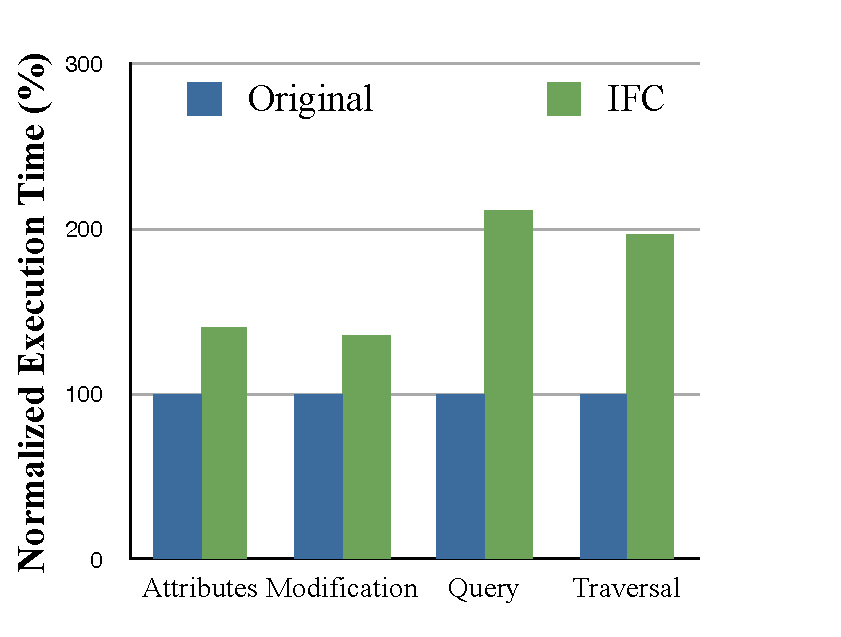
\includegraphics[width=0.8\linewidth]{chapters/browser/DOMCore.pdf}
%   \caption{Overheads of IFC on Dromaeo DOM Core Benchmark Tests}
%   \label{fig:dom}
% \end{figure}

% \begin{figure}
%   \centering
%     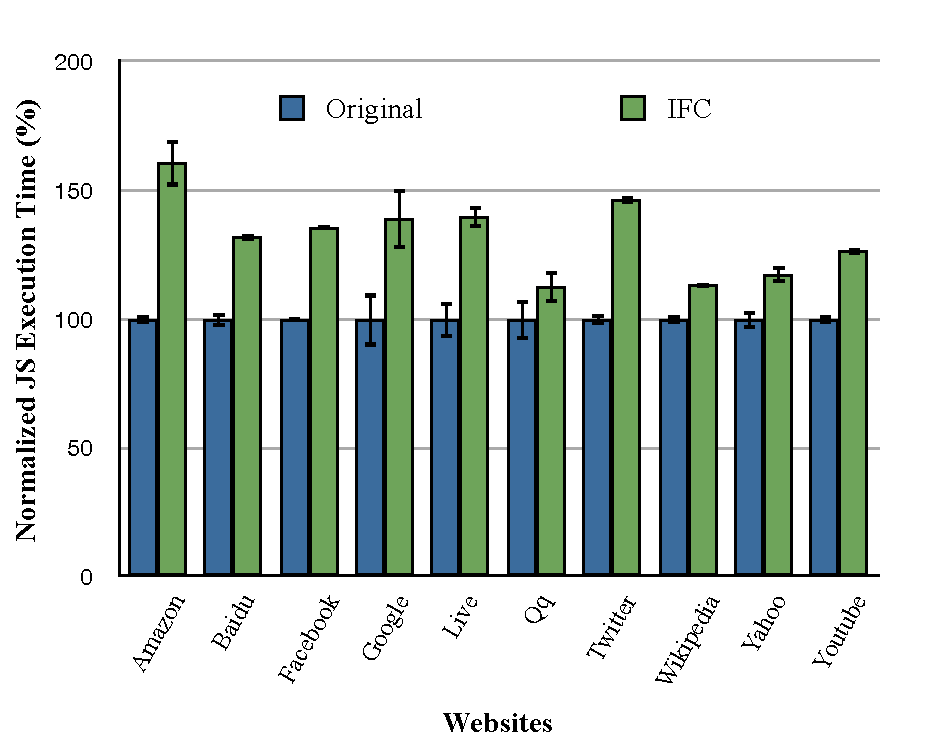
\includegraphics[width=\linewidth]{chapters/browser/Macro.pdf}
%   \caption{Overheads of IFC on Alexa Top 10 Websites}
%   \label{fig:macro}
% \end{figure}


% \begin{figure}
%   \centering
%     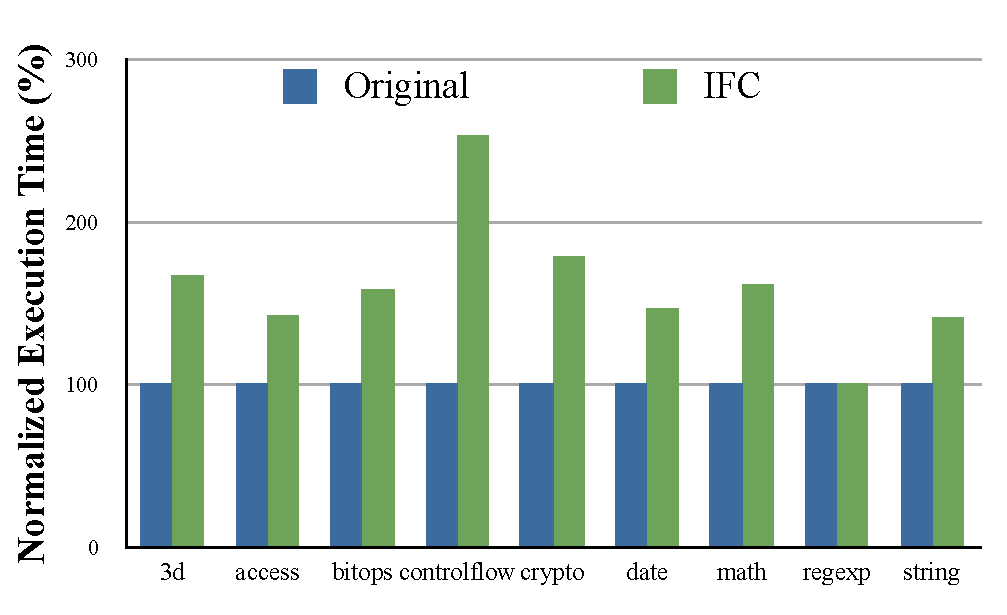
\includegraphics[width=\linewidth]{chapters/browser/SunSpider.pdf}
%   \caption{Overheads of IFC on SunSpider JavaScript Benchmark Tests}
%   \label{fig:js}
% \end{figure}

% The instrumentation is evaluated on the Dromaeo DOM Core
% benchmark~\cite{dromaeo}, which measures the performance of various
% operations on the DOM. The average overhead is approximately 71\% over
% the uninstrumented browser. Normalized overheads on different kinds of
% tests are shown in Figure~\ref{fig:dom} (standard deviations on
% individual tests were small, ranging from 0.17\% to 8.45\%). To get a
% more realistic evaluation, the instrumentation was also tested on the
% Alexa Top 10 websites~\cite{alexa}. The execution time of JavaScript
% was measured that loads initially on each website’s front page,
% without any user interaction. The graph in Figure~\ref{fig:macro}
% shows normalized execution time. Error bars are standard
% deviations. The average overhead is approximately 32\% and the worst 
% overhead is around 60\%. Note that both the Dromaeo and Alexa tests
% are very performance-intensive and do not count common browser delays
% like network communication and page rendering in the
% baseline. Compared to a baseline that includes these delays, our
% overheads are negligible. Finally, the very popular SunSpider
% benchmark~\cite{sunspider} was also run. SunSpider is a pure JS
% benchmark that does not cover events or the DOM. Results are shown in
% Figure~\ref{fig:js}. Although the overheads of IFC vary from test to
% test, the average overheads over the baseline uninstrumented
% interpreter is about 45\%. 

%% Tables~\ref{table:rap} and~\ref{table:eap} records the evaluation
%% results for the different applications in the three configurations. In 
%% general, the average overhead for page-load varies from 4.16\% to 40\% 
%% for \textbf{IFC}. \textbf{\sys} adds an overhead of about 2.79\% to
%% 29.16\% on top of it. The average overhead for JavaScript execution 
%% varies from 16\% to 83\% for \textbf{IFC} on top of
%% \textbf{Base}. To this overhead, the execution of
%% policy handlers (\textbf{{\sys}}) adds another 4\% to 29\%, relative
%% to \textbf{Base}. (See Appendix for a detailed analysis of the evaluation.)

% Table~\ref{table:rap} records the evaluation results for the
% real-world applications in the three configurations. In 
% general, the average overhead for page-load varies from 13\% to 40\%
% for \textbf{IFC}. \textbf{\sys} adds a small overhead of about 2.79\% to
% 3.18\% on top of it. 

% Table~\ref{table:eapl} shows the results for the four example programs.
% The overhead of the page load time of \textbf{IFC} with respect to
% \textbf{Base} varies from 4.16\% to 7.69\%. The overhead added
% by \sys with respect to \textbf{Base} varies from 12.19\% to
% 29.16\%. The average overhead for JavaScript execution 
% varies from 16\% to 83\% for \textbf{IFC} on top of
% \textbf{Base}. To this overhead, the execution of
% policy handlers (\textbf{{\sys}}) adds another 13\% to 29\%, relative
% to \textbf{Base}. 

% The average time for loading the website (over 20 runs) on
% \textbf{Base} was 303 ms with a standard deviation of about 3.58\%. For
% \textbf{IFC}, the average time was 429 ms with a standard deviation of
% about 2.3\% adding an overhead of about 41.5\% over
% \textbf{Base}. The average time for loading the website including the
% policy (\textbf{\sys}), was 441 ms with a standard deviation of about
% 3.82\%. The ovehead of \textbf{\sys} over \textbf{Base} is 45.5\%
% and over \textbf{IFC} is just 2.79\%.

% The average time for loading the website (over 20 runs) on
% \textbf{Base} was 2151 ms with a standard deviation of about 2.59\%. For
% \textbf{IFC}, the average time was 2422 ms with a standard deviation of
% about 1.08\% adding an overhead of about 12.59\% over
% \textbf{Base}. The average time for loading the website including the
% policy (\textbf{\sys}), was 2499 ms with a standard deviation of about
% 3.02\%. The ovehead of \textbf{\sys} over \textbf{Base} is 16.17\%
% and over \textbf{IFC} is 3.18\%.

% \TODO{Figure in appendix now}

%% \begin{table}[tbp]
%% \centering
%% \begin{tabular}{ | C{2cm} || C{1.5cm} | C{1.5cm} | C{1.5cm} || C{1.5cm} | C{1.5cm} | C{1.5cm} |}
%% \hline
%% \multicolumn{1}{|c||}{ } &
%% \multicolumn{3}{ c ||}{JavaScript Execution Time} &
%%                                                        \multicolumn{3}{
%%                                                          c |}{Page Load Time} \\
%% \hline
%%  \multicolumn{1}{|c||}{Applications} & Base & IFC & \sys & Base & IFC & \sys \\
%% \hhline{|=#=|=|=#=|=|=|} 
%%  \multicolumn{1}{|c||}{Password} & 79.5 & 115.5 & 126 & 303 & 429 & 441 \\  
%% \hline
%%  \multicolumn{1}{|c||}{Analytics} & 273.4 & 375.1 & 386.1 & 2151 & 2422 & 2499 \\ 
%% \hline
%% \end{tabular}
%% \caption{Real Applications Performance (time in ms)}
%% \label{table:rap}
%% \end{table}

% \begin{table}
% \centering
% \begin{tabular}{ | c | c | c | c |}
% \hline
%  Applications & Base & IFC & \sys \\
% \hline
% \hline
%   Analytics & 2151 & 2422 & 2499 \\ 
% \hline
%   Password & 303 & 429 & 441 \\  
% \hline
% \end{tabular}
% \caption{Real applications - Page Load Time (in ms)}
% \label{table:rapl}
% \end{table}

%% \begin{table}[tbp]
%% \centering
%% \begin{tabular}{ | C{2cm} || C{1.5cm} | C{1.5cm} | C{1.5cm} || C{1.5cm} | C{1.5cm} | C{1.5cm} |}
%% \hline
%% \multicolumn{1}{|c||}{ } &
%% \multicolumn{3}{ c ||}{JavaScript Execution Time} &
%% \multicolumn{3}{ c |}{Page Load Time} \\
%% \hline
%%  Example Applications & Base & IFC & \sys & Base & IFC & \sys \\
%%   \hhline{|=#=|=|=#=|=|=|} 
%%   PSC & 2430 & 2918 & 2989 & 16 & 17 & 19 \\  
%% \hline
%%   Converter & 3443 & 4361 & 5368 & 41 & 43 & 46 \\ 
%% \hline
%%   Presence & 1504 & 1737 & 1911 & 24 & 25 & 31 \\
%% \hline
%%   Coordinate & 1780 & 2095 & 2414 & 26 & 28 & 30 \\
%% \hline
%% \end{tabular}
%% \caption{Example Applications Performance (time in ms)}
%% \label{table:eap}
%% \end{table}

% \begin{table}
% \centering
% \begin{tabular}{ | c | c | c | c |}
% \hline
%  Example Applications & Base & IFC & \sys \\
% \hline
% \hline
%   Currency Converter & 3443 & 4361 & 5368 \\ 
% \hline
%   Password Strength Checker & 2430 & 2918 & 2989 \\  
% \hline
%   Presence & 1504 & 1737 & 1911 \\
% \hline
%   Coordinate & 1780 & 2095 & 2414 \\
% \hline
% \end{tabular}
% \caption{Example applications - JavaScript Execution Time (in ms)}
% \label{table:eapl}
% \end{table}

% Figure~\ref{fig:perf} shows the JavaScript execution times averaged
% over five runs for each program in each configuration. Standard
% deviations were small, no more than 3\%, except in the currency
% converter {\textbf{\sys}} line (7\%). 
% The overhead of taint tracking
% (\textbf{IFC}) over the baseline (\textbf{Base}) varies from 16\% in
% analytics presence to 83\% in password strength. This overhead is
% higher for scripts that perform more arithmetic and logical operations
% and our measurements are consistent with those from our prior work,
% which measured the same overhead on standard benchmarks~\cite{post14,csf15}. 
% To this overhead, the execution of
% policy handlers (\textbf{{\sys}}) adds another 13\% to 29\%, relative
% to \textbf{Base}. This policy overhead is proportional to the ratio of
% the work done in the policy code to other JavaScript. Most of the cost
% in policy code comes from executing native functions like
% \texttt{getElementbyId()}, which is used to find the DOM element whose
% label must be set or to which a policy handler must be attached. The
% figure plotting the JavaScript execution times for each of the examples
% is included in the Appendix.

% We note that this is a very challenging baseline for {\sys} and the
% experiment measures overheads very conservatively. The scripts in both
% sub-examples of Example~3 do almost nothing. The scripts in Examples~1
% and Example~2 are slightly longer, but are still much simpler than
% real scripts. On real, and longer scripts, the relative overheads of
% evaluating the policy handlers will be significantly lower. Moreover,
% our baseline does not include other browser costs, such as the cost of
% parsing, page loading and rendering, and network delays. In fact, the
% overheads induced by both taint tracking and policy handlers are too
% small to be perceived by the browser's user. They do not exceed 2.56ms
% across all interactions in any of the four experiments.

% The overhead of the page load time of \textbf{IFC} with respect to
% \textbf{Base} is 4.8\%, 6.25\%, 4.16\%, and 7.69\%. The overhead added
% by \sys with respect to \textbf{Base} is 12.19\%, 18.75\%, 29.16\%,
% and 15.38 \%. 

% The standard deviation varies from 2.3 \% to 4.3 \% for
% \textbf{Base}, 2.85\% to 4.17\% for \textbf{IFC} and 3.6\% to 7.4\%
% for \sys.

%% The performance measure are performed on
%% on a 3.2GHz Quad-core Intel Xeon processor with 8GB RAM, running Mac OS X
%% version 10.7.4. We extend our previous instrumentation of taint tracking
%% from~\cite{csf15} which is based on WebKit build \#r122160 and works with the
%% Safari web browser, version 6.0. As the major changes to the browser were
%% confined to the event handling mechanism of the browser, running the JavaScript
%% benchmarks produced a similar moderate performance overhead as shown in our
%% earlier work. The additional overhead of executing the policy code is dependent
%% on the size of the policy code. We perform two kinds of performance experiments.

%% First, we measure the overhead of taint tracking by running our examples (not
%% containing policy) on the instrumented browser against the same examples (not
%% containing policy) on the unmodified browser. As can be seen in
%% Figure~\ref{fig:taintOverhead} the average percentage overhead of taint tracking
%% is around ...

%% Second, we measure the overhead due to the changes introduced by the inlcusion
%% of the policy. The average percentage overhead per example is shown in
%% Figure~\ref{fig:policyOverhead}.

% The average time for
% loading the two websites on \textbf{Base} was 356.2 ms and 2196.4 ms, 
% respectively, and with \textbf{\sys}, the average time for loading the
% two websites along with the policies was 415 ms and 2477 ms,
% respectively.  


%% To evaluate the practicality and usability of the model, we conducted
%% an anecdotal study with a few students from the university. The
%% students were given a set of four exercises (based on the examples
%% presented before) to write security policies for and the documentation
%% related to the additional set of APIs that they could use for specifying these
%% policies. They also had access to a running prototype of our
%% implementation where they could check the policies specified by them
%% against the requirement. To summarise the results: we found that the
%% students who were knowledgable with JavaScript and HTML programming
%% and did not have any prior knowledge of information flow control
%% were able to specify correct policies for almost all exercises with
%% the exception of those that required the execution context to be
%% set. The students who had knowledge of both information flow
%% control and JavaScript and HTML programming were able to specify
%% correct policies for all the exercises. The students who had basic
%% knowledge of programming with JavaScript and HTML but had knowledge of
%% IFC weren't able to specify the correct policy in one out of the four
%% cases that required a non-trivial JavaScript specification. The other
%% major problem which the students had was that the documentation was
%% not extensive enough but with some discussion they were able to
%% understand the functionality of the model better. Overall, we found
%% that the specification of policies would in general require a good
%% knowledge of JavaScript and HTML programming but very basic knowledge
%% of IFC, which evaluates the usability of our model positively
%% considering the fact that web developers only need to have some basic
%% training of IFC to be able to specify the required security policies.
